\justifying \small 

\textcolor{orange}{\#define \_\_GLIBC\_INTERNAL\_STARTING\_HEADER\_IMPLEMENTATION} 
\textcolor{orange}{\#include <bits/libc-header-start.h>} 
\textcolor{white}{\_\_BEGIN\_DECLS} 
\textcolor{orange}{\#define \_\_need\_size\_t} 
\textcolor{orange}{\#define \_\_need\_NULL} 
\textcolor{orange}{\#include <stddef.h>} 
\textcolor{orange}{\#define \_\_need\_\_\_va\_list} 
\textcolor{orange}{\#include <stdarg.h>} 
\textcolor{orange}{\#include <bits/types.h>} 
\textcolor{orange}{\#include <bits/types/\_\_fpos\_t.h>} 
\textcolor{orange}{\#include <bits/types/\_\_fpos64\_t.h>} 
\textcolor{orange}{\#include <bits/types/\_\_FILE.h>} 
\textcolor{orange}{\#include <bits/types/FILE.h>} 
\textcolor{orange}{\#include <bits/types/struct\_FILE.h>} 
\textcolor{orange}{\#ifdef \_\_USE\_GNU} 
\textcolor{orange}{\# include <bits/types/cookie\_io\_functions\_t.h>} 
\textcolor{orange}{\#endif} 
\textcolor{orange}{\#define \_IOFBF 0		} 
\textcolor{orange}{\#define \_IOLBF 1		} 
\textcolor{orange}{\#define \_IONBF 2		} 
\textcolor{orange}{\#define BUFSIZ 8192} 
\textcolor{orange}{\#define EOF (-1)} 
\textcolor{orange}{\#define SEEK\_SET	0	} 
\textcolor{orange}{\#define SEEK\_CUR	1	} 
\textcolor{orange}{\#define SEEK\_END	2	} 
\textcolor{orange}{\#ifdef \_\_USE\_GNU} 
\textcolor{orange}{\# define SEEK\_DATA	3	} 
\textcolor{orange}{\# define SEEK\_HOLE	4	} 
\textcolor{orange}{\#endif} 
\textcolor{orange}{\#if defined \_\_USE\_MISC || defined \_\_USE\_XOPEN} 
\textcolor{orange}{\# define P\_tmpdir	"/tmp"} 
\textcolor{orange}{\#endif} 
\textcolor{orange}{\#include <bits/stdio\_lim.h>} 
\textcolor{cyan}{extern} 
\textcolor{white}{FILE} 
\textcolor{yellow}{*} 
\textcolor{white}{stdin} 
\textcolor{magenta}{;} 
\textcolor{cyan}{extern} 
\textcolor{white}{FILE} 
\textcolor{yellow}{*} 
\textcolor{white}{stdout} 
\textcolor{magenta}{;} 
\textcolor{cyan}{extern} 
\textcolor{white}{FILE} 
\textcolor{yellow}{*} 
\textcolor{white}{stderr} 
\textcolor{magenta}{;} 
\textcolor{orange}{\#define stdin stdin} 
\textcolor{orange}{\#define stdout stdout} 
\textcolor{orange}{\#define stderr stderr} 
\textcolor{orange}{\#if defined \_\_USE\_MISC || defined \_\_USE\_XOPEN} 
\textcolor{cyan}{extern} 
\textcolor{cyan}{char} 
\textcolor{yellow}{*} 
\textcolor{white}{tempnam} 
\textcolor{magenta}{(} 
\textcolor{cyan}{const} 
\textcolor{cyan}{char} 
\textcolor{yellow}{*} 
\textcolor{white}{\_\_dir} 
\textcolor{magenta}{,} 
\textcolor{cyan}{const} 
\textcolor{cyan}{char} 
\textcolor{yellow}{*} 
\textcolor{white}{\_\_pfx} 
\textcolor{magenta}{)} 
\textcolor{white}{\_\_THROW} 
\textcolor{white}{\_\_attribute\_malloc\_\_} 
\textcolor{white}{\_\_wur} 
\textcolor{magenta}{;} 
\textcolor{orange}{\#endif} 
\textcolor{orange}{\#include <stdio.h>} 
\textcolor{orange}{\#define DIRECTIVA "Hyderabad" } 
\textcolor{cyan}{int} 
\textcolor{white}{main} 
\textcolor{magenta}{(} 
\textcolor{magenta}{)} 
\textcolor{magenta}{\{} 
\textcolor{white}{printf} 
\textcolor{magenta}{(} 
\textcolor{green}{"\%s "} 
\textcolor{magenta}{,} 
\textcolor{white}{DIRECTIVA} 
\textcolor{magenta}{)} 
\textcolor{magenta}{;} 
\textcolor{cyan}{return} 
\textcolor{green}{0} 
\textcolor{magenta}{;} 
\textcolor{magenta}{\}} 




\begin{frame}{Histograma Tokens Usados} 
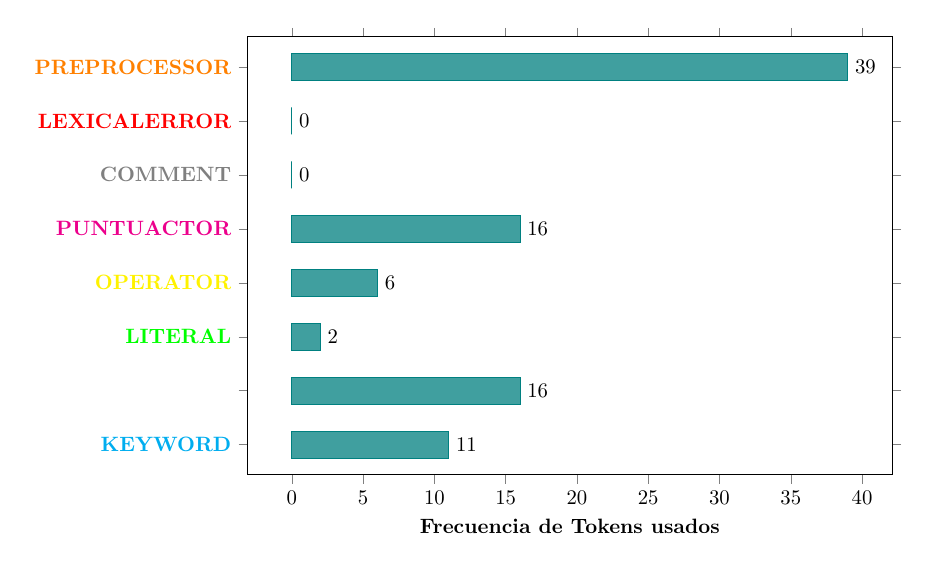
\begin{tikzpicture}[scale=0.75] % tamaño 
\begin{axis}[xbar,tick align=outside, 
    width=12.5cm,       % largo 
    height=9cm,       % altura 
    bar width={13pt},   % grosor linea 
    enlargelimits=0.08, % cercania a linea 
    nodes near coords, 
    nodes near coords align=horizontal, 
    point meta=x * 1, % The displayed number. 
    xlabel=\textbf{Frecuencia de Tokens usados}, 
    ytick={0,...,7}, 
    yticklabels={ 
        \textcolor{cyan}{\textbf{KEYWORD}},         % POSITION 0 
        \textcolor{white}{\textbf{IDENTIFIER}},     % POSITION 1 
        \textcolor{green}{\textbf{LITERAL}},        % POSITION 2 
        \textcolor{yellow}{\textbf{OPERATOR}},      % POSITION 3 
        \textcolor{magenta}{\textbf{PUNTUACTOR}},   % POSITION 4 
        \textcolor{gray}{\textbf{COMMENT}},         % POSITION 5 
        \textcolor{red}{\textbf{LEXICALERROR}},     % POSITION 6 
        \textcolor{orange}{\textbf{PREPROCESSOR}}   % POSITION 7 
    }] 
\addplot 
[draw=teal,fill=teal!75] 
coordinates {(11,0) (16,1) (2,2) (6,3) (16,4) (0,5) (0,6) (39,7)}; 
\end{axis}
\end{tikzpicture}
\end{frame}
